\documentclass[12pt, oneside, a4paper]{article}
\usepackage[T1]{fontenc}
\usepackage[utf8]{inputenc}

%\usepackage[cp1251]{inputenc} % кодировка
\usepackage[english, russian]{babel} % Русские и английские переносы

\usepackage{cite}              % для корректного оформления литературы

\usepackage{graphicx}          % для включения графических изображений
\usepackage{enumitem}

\setlength{\emergencystretch}{3em}
\usepackage[hyphens]{url}
\usepackage[misc,geometry]{ifsym}

\usepackage[usenames]{xcolor}
\usepackage{soul}

\usepackage{amsmath}
\usepackage{amssymb}

\usepackage{algorithm}
\usepackage{algorithmic}

\usepackage{listings}

\usepackage{pavt-ru}
%\usepackage{pgfplots}
%\pgfplotsset{compat=1.9}
\usepackage{listings}


\lstset{
language=C,                 % выбор языка для подсветки (здесь это С)
basicstyle=\scriptsize\ttfamily, % размер и начертание шрифта для подсветки
numbers=left,               % где поставить нумерацию строк (слева\справа)
numberstyle=\tiny,           % размер шрифта для номеров строк
stepnumber=0,                   % размер шага между двумя номерами строк
numbersep=5pt,                % как далеко отстоят номера строк от подсвечиваемого кода
backgroundcolor=\color{white}, % цвет фона подсветки - используем \usepackage{color}
showspaces=false,            % показывать или нет пробелы специальными отступами
showstringspaces=false,      % показывать или нет пробелы в строках
showtabs=false,             % показывать или нет табуляцию в строках
frame=single,              % рисовать рамку вокруг кода
tabsize=2,                 % размер табуляции по умолчанию равен 2 пробелам
captionpos=t,              % позиция заголовка вверху [t] или внизу [b] 
breaklines=true,           % автоматически переносить строки (да\нет)
breakatwhitespace=false, % переносить строки только если есть пробел
escapeinside={\%*}{*)}   % если нужно добавить комментарии в коде
}

%Содержимое документа
\begin{document}

\title{Отчет о выполнении 1 задания практикума кафедры СКИ}
\authors{Р.М.~Куприй, 323 группа}
\organizations{Факультет ВМК МГУ имени М.В.~Ломоносова}

\section{Задание}

По заданию написана программа для решения системы линейных уравнений $Ax = b$, с плотной матрицей $A$ и векторами $x$, $b$. Алгоритм решения системы уравнений состоит из приведения матрицы к верхнетреугольному виду методом отражений Хаусхолдера, а затем решение получившейся системы методом обратного хода Гаусса.

Метод отражений Хаусхолдера заключается в последовательном умножении матрицы разложения на плотную матрицу $A$ и на вектор правой части. При этом, матрица разложения не хранится в явном виде, поскольку достаточно на каждой итерации разложения вычислять и хранить один вектор Хаусхолдера. Для более эффективной работы кэша, матрица $A$ хранится по столбцам.

В программе реализована параллельная версия алгоритма, с использованием технологий OpenMP.

\section{Методика тестирования}

В программе замеряется время разложения матрицы и время решение системы обратным ходом Гаусса, общее время есть сумма этих двух составляющих. Для верификации результатов вычисляется невязка решения: $||Ax - b||$, а также при известном решении системы -- невязка ошибки: $||x - solution||$. Примером известного решения может быть единичный вектор $x$, который возникает тогда, когда вектор $b$ составлен из сумм строк матрицы $A$.

Для тестирования производительности использовалась параллельная вычислительная система Polus, с 3 вычислительными узлами, в каждом из которых 2 10~ядерных процессора IBM POWER8. Для компиляции использовался компилятор \texttt{xlc++} с флагом опимизации -O5. Запуски проводились с привязкой нитей к физическим ядрам с помощью специального скрипта на языке python.

Программа запускалась 6 раз для каждого замера, с выбором наименьшего времени исполнения, чтобы исключить выбросы. Получены резльтаты для плотных матриц разного размера, при использовании 1, 2, 4, 8, 32, 64 и 128 нитей соотвественно.

\section{Оценки эффективности OpenMPI программы}

Для каждого набор входных данных приведены графики общего времени решения системы, ускорения и эффективности.

Для небольшой матрицы, размером 1000 строк, максимальное ускорение достигается на 32 нитях, при этом эффективность резко падает ниже 80\% уже при использовании более 8 нитей (Графики~\ref{fig:m1000}). Это связано с тем, что при увеличении числа нитей, нельзя привязать все нити к ядрам одного процессора. Либо используется несколько процессоров, либо на одно физическое ядро приходится две нити. Конкуренция между нитями за вычислительные юниты процессора, а также издержки на создание нитей значительно возрастают с ростом числа нитей.

\begin{figure}[h!]
\center{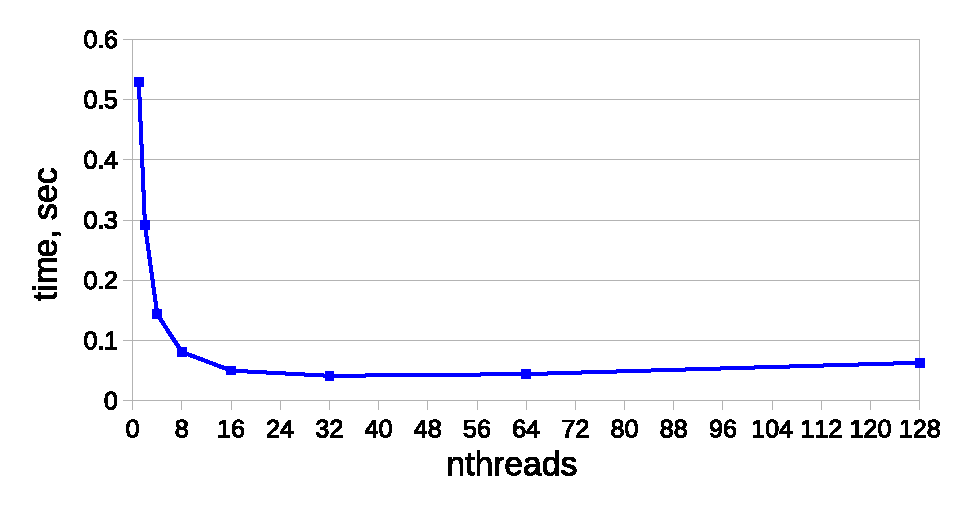
\includegraphics[width=12cm]{./pics/time1000.eps}}
\center{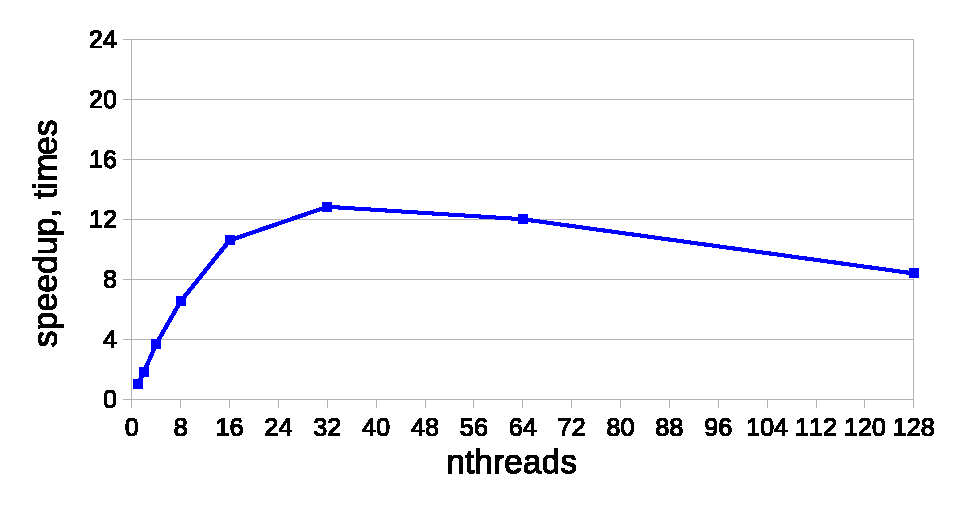
\includegraphics[width=12cm]{./pics/speedup1000.eps}}
\center{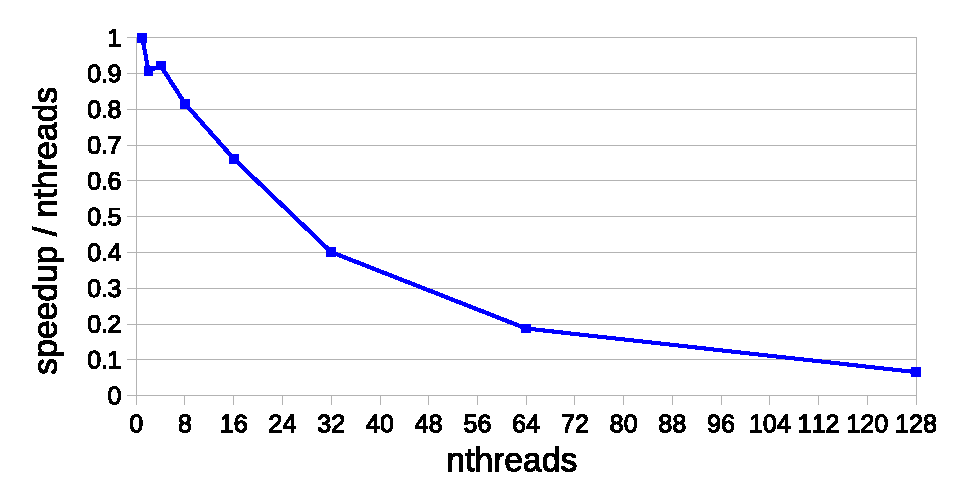
\includegraphics[width=12cm]{./pics/efficiency1000.eps}}
\caption{Результаты распараллеливания программы для матрицы размером 1000 строк; верхний график -- времена исполнения, срений -- достигаемое ускорение, нижний -- эффективность ускорения работы программы}
\label{fig:m1000}
\end{figure}

В следующем наборе измерений использовалась матрица размером 4000 строк. C ростом объема данных растёт ресурс параллелизма, который можно использовать. Это повышает эффективность распараллеливания. Так, при использовании до 16 нитей включительно, эффективность ускорения сохраняется выше 80\%. Однако с дальнейшим ростом числа нитей, эффективгость распараллеливания снова значительно падает, поскольку нельзя закрепить все нити за физическими ядрами двух процессоров - одного узла (Графики~\ref{fig:m4000}).

\begin{figure}[h!]
\center{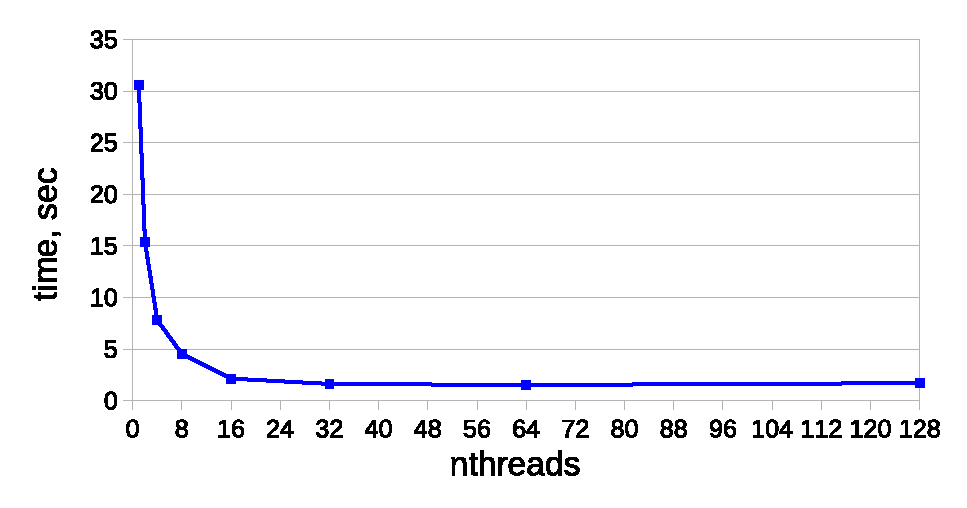
\includegraphics[width=12cm]{./pics/time4000.eps}}
\center{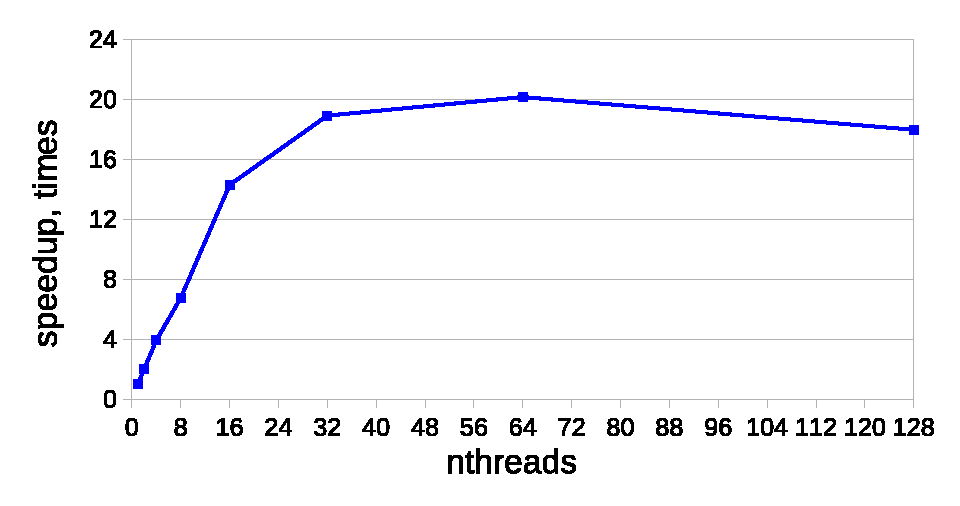
\includegraphics[width=12cm]{./pics/speedup4000.eps}}
\center{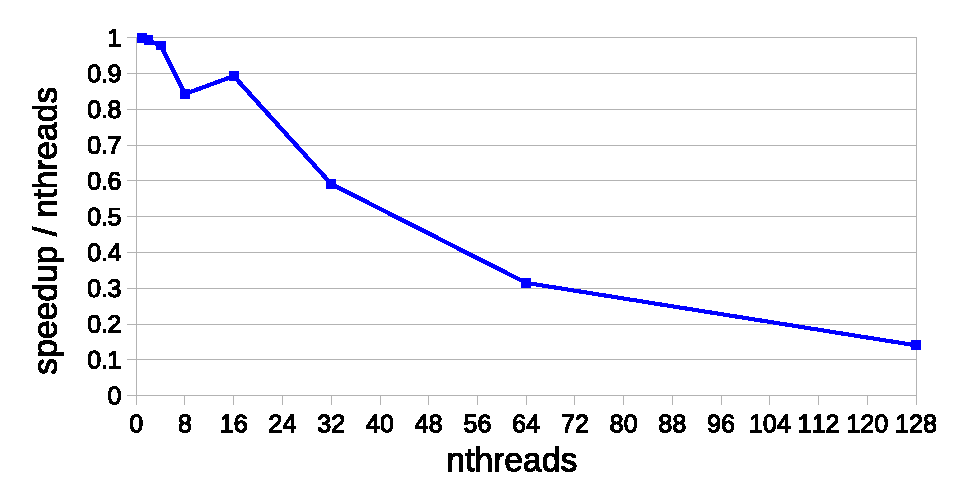
\includegraphics[width=12cm]{./pics/efficiency4000.eps}}
\caption{Результаты распараллеливания программы для матрицы размером 4000 строк; верхний график -- времена исполнения, срений -- достигаемое ускорение, нижний -- эффективность ускорения работы программы}
\label{fig:m4000}
\end{figure}

Последний набор данных использует матрицу размером 6000 строк. На нём уже не получается достигнуть такого же значительного ускорения, как на среднем наборе данных (Графики~\ref{fig:m6000}). Это может быть негативным влиянием комбинации факторов -- нехватки физических ядер для размещения всех нитей на своих ядрах и большого объема данных необходимых для распределения между нитями.

\begin{figure}[h!]
\center{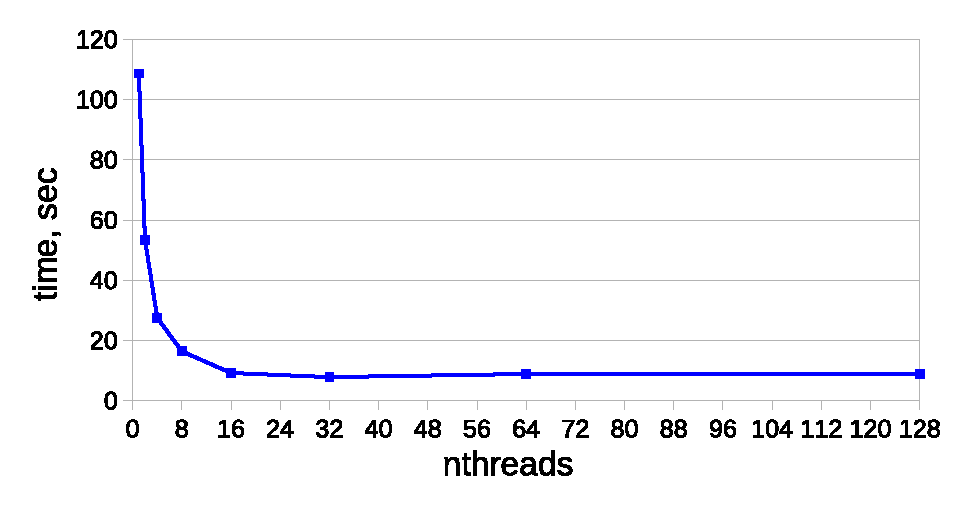
\includegraphics[width=12cm]{./pics/time6000.eps}}
\center{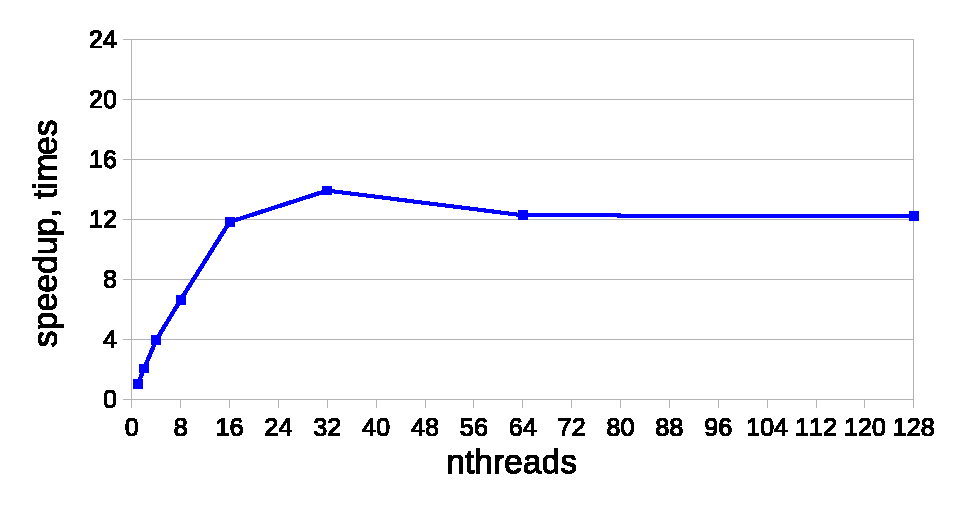
\includegraphics[width=12cm]{./pics/speedup6000.eps}}
\center{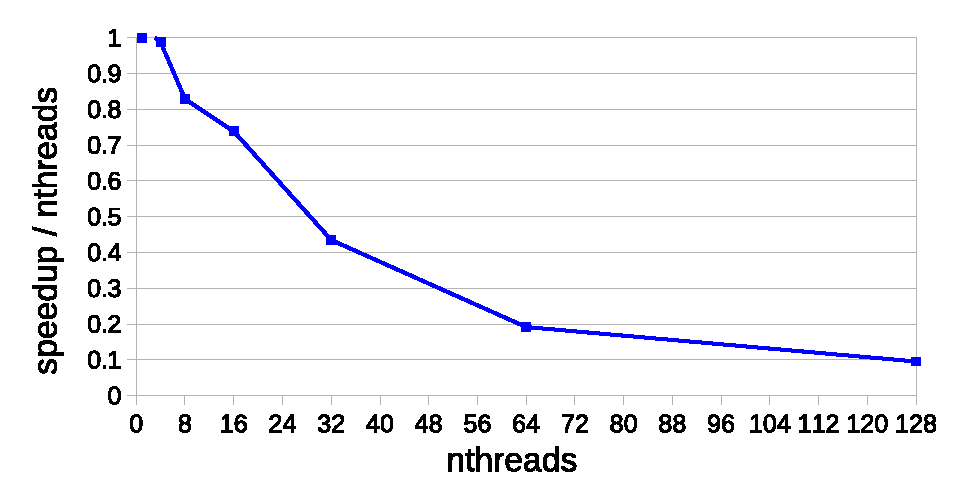
\includegraphics[width=12cm]{./pics/efficiency6000.eps}}
\caption{Результаты распараллеливания программы для матрицы размером 6000 строк; верхний график -- времена исполнения, срений -- достигаемое ускорение, нижний -- эффективность ускорения работы программы}
\label{fig:m6000}
\end{figure}

\end{document}